\section{Implementación de atractor Determinístico - Estocástico}

\subsection{Introduction}

En los últimos treinta años, los sistemas caóticos han producido una revolución en nuestra visión de la naturaleza ya que tienen dos características contrastantes:
(1) son deterministas porque un modelo matemático determina su dinámica, pero
(2) debido a su sensibilidad a las condiciones iniciales, se pierde la predicción a largo plazo y, en consecuencia, pueden incluirse en la clase de sistemas estocásticos que se estudian mediante herramientas estadísticas.
En realidad, si los sistemas caóticos pudieran implementarse con una precisión infinita, serían deterministas en sentido estricto, pero la precisión infinita es un ideal imposible de alcanzar en la electrónica digital.

Esta \emph{dualidad determinista-estocástica} hace que los sistemas caóticos sean especialmente interesantes para las aplicaciones de ingeniería, en la medida en que las señales generadas pueden usarse como ruidos controlados en una amplia gama de aplicaciones.
Sin embargo, las secuencias caóticas realmente presentan correlaciones internas no lineales, lo que las hace inadecuadas para ser utilizadas como "buenas" PRNG.
Es necesario utilizar técnicas de aleatorización para mejorar la aleatoriedad de la serie \cite{DeMicco2008}.

En aplicaciones digitales, el tiempo y la variable de estado tienen valores discretos.
La discretización de tiempo impone el uso de un algoritmo para aproximar las ecuaciones diferenciales de tiempo continuo que modelan el sistema.
El algoritmo más simple es el método de Euler de primer orden en el que los diferenciales se reemplazan directamente por incrementos finitos.
Los algoritmos más elaborados, como los algoritmos de paso variable Runge-Kutta de cuarto orden (o superior), hacen que el sistema discreto evolucione más cerca del sistema continuo, pero con mayores requisitos de recursos de hardware y tiempos de cálculo.
En consecuencia, deben usarse solo si la exactitud es un requisito de la aplicación específica.
Este no es el caso en PRNG, donde la aleatoriedad es la característica principal que debe garantizarse.

Para hacer los cálculos aritméticos, las computadoras deben representar internamente las señales por un número finito de bits, esto significa que los valores se describen usando aritmética de precisión finita.
Esta restricción puede ser crítica para un sistema caótico ya que es extremadamente sensible a la aritmética empleada e incluso puede perder su comportamiento caótico.

En este capítulo, implementamos un oscilador discreto de Lorenz obtenido mediante el uso del algoritmo de primer orden de Euler y tres estándares de representación diferentes.
Además aplicamos técnicas de aleatorización a las variables de estado para obtener un PRNG en tiempo real.
El objetivo de este trabajo es estudiar la influencia del procedimiento de discretización en la dinámica del sistema.
En \cite{DeMicco2010} se estudió el grado de estocasticidad de un sistema caótico determinista mediante su implementación en coma flotante de precisión simple (32 bits).

La determinación del grado de estocasticidad tiene como objetivo proporcionar una metodología de diseño optimizada para la utilidad prevista dada al sistema caótico.
Así, por ejemplo, hay aplicaciones que requieren que el sistema caótico reemplace un sistema estocástico (criptografía \cite{Fernandez2003}, generadores de secuencia para difundir comunicaciones de espectro \cite{Setti2004, DeMicco2007B}, generadores de números pseudoaleatorios \cite{Kocarev2003, Larrondo2006, DeMicco2009}, reducción de la interferencia electromagnética \cite{Callegari2003A}, etc.).
Por otro lado, algunas aplicaciones requieren previsibilidad a largo plazo, por ejemplo para reproducir el sistema caótico de la manera más precisa posible, este es el caso de las comunicaciones analógicas que usan portadores de sincronización caóticos \cite{Kocarev1995, Hidalgo2001}.

Otro problema es la determinación exacta del período de la secuencia pseudoaleatoria.
Para generadores que se basan en operaciones lineales, el problema se ha estudiado en profundidad y existen criterios de diseño bien conocidos para obtener dispositivos de ciclo máximo.
Ejemplos de algoritmos lineales son: el algoritmo Mersenne Twister que es un generador de números aleatorios muy rápido de período $T = 2^{19937} - 1$ \cite{Matsumoto1998} y Multiply-With-Carry (MWC), un método inventado por George Marsaglia para la generación de secuencias de enteros aleatorios basados en un conjunto inicial de dos a muchos miles de valores de semilla elegidos al azar, presenta períodos inmensos, que van desde alrededor de $2 ^ {60}$ a $2 ^ {2000000}$ \cite{Marsaglia1991}.
Sin embargo, desde el punto de vista criptográfico son débiles.
Cuando se trata de aplicaciones criptográficas, no se recomiendan métodos lineales para generar secuencias pseudoaleatorias (como LFSR, LCG o sus combinaciones adecuadas), ya que algoritmos eficientes para predecir la secuencia sobre la base de una secuencia de observación relativamente corta están a disposición \cite{Boyar1989, Plumstead1982}.
Por otro lado, para la mayoría de las familias de generadores no lineales, el problema parece ser intratable y, con pocas excepciones, no suele existir una evaluación analítica de sus períodos \cite{kocarev2011}.

Elegimos el sistema caótico de Lorenz porque es un sistema ampliamente estudiado y también ha sido implementado por otros autores con diferentes metodologías \ cite {Asseri2002, Azzaz2009, Azzaz2010}.
Por ejemplo, en \ cite {Asseri2002}, se implementó un oscilador caótico Lorenz mediante una caja de herramientas del Generador de Sistemas Xilinx que funciona bajo $ MATLAB-Simulink ^\copyright $.
Esta caja de herramientas convierte el modelo MATLAB-Simulink en el modelo de Xilinx System Generator.
Luego se obtiene el código VHDL.
Como es una operación automática, no permite ciertos cambios específicos y presenta algunas limitaciones.
La operación de integración se aproximó con el algoritmo de Euler, utilizando bloques de suma y retardo. La implementación propuesta en \ cite {Azzaz2009} y \ cite {Azzaz2010} usa $ RK4 $ en una arquitectura de punto fijo de $ 32- $ bit.
La aplicación considerada fue la generación de clave aleatoria caótica para el cifrado de flujo de datos.

In this paper $Quartus$ II $7.2^\copyright$ development software is used to generate the VHDL hardware description language and the physical implementation is made on the development board $Altera^\copyright$ Cyclone III $EP3C120$.
Three representations are studied:
1)  floating-point IEEE $754$ standard,
2) decimal fixed point, and 
3) integer arithmetics \cite{Gonzalez2003}.
Each representation involves a different number of bits.
We consider two floating point representations for the standards single or double, with $32$ and $64$ bits respectively to represent the sign, the exponent and the mantissa;
decimal fixed point arithmetics uses $p$ bits to represent the integer part and $m$ bits to represent the fractional part.
We considered $32$ and $64$ bits fixed point representations with $9$ bits for the integer part and $1$ bit for the sign and the remaining $22$ or $54$ bits for the fractional part.
In the $k$ bits integer arithmetics the alphabet has $2^k$ symbols.
We considered $k=54$.

En esta sección se utilizó el software \textit{QuartusII\textsuperscript{\copyright} 7.2} para generar el lenguaje de descripción de hardware VHDL y la implementación física se realiza en la placa de desarrollo \textit{Altera\textsuperscript{\copyright} Cyclone III EP3C12}.
Tres representaciones numéricas son estudiadas:
1) punto flotante IEEE 754 estándar,
2) punto fijo decimal, y
3) aritmética entera \cite{Gonzalez2003}.
Cada representación implica una cantidad diferente de bits.
Consideramos dos representaciones de coma flotante para los estándares simple o doble, con $32$ y $64$ bits respectivamente para representar el signo, el exponente y la mantisa;
La aritmética decimal de punto fijo usa $p$ bits para representar la parte entera y $m$ bits para representar la parte fraccional.
Consideramos representaciones de punto fijo de $32$ y $64$ bits con $9$ bits para la parte entera y $1$ bit para el signo y los $22$ o $54$ bits restantes para la parte fraccionaria.
En los aritméticos enteros $k$ bits el alfabeto tiene $2^k$ símbolos.
Consideramos $k=54$.

Para cuantificar la aleatoriedad del sistema, se utiliza el conjunto de pruebas DIEHARD de Marsaglia.
Estas pruebas han sido ampliamente utilizadas en la literatura abierta y son muy efectivas para clasificar sistemas determinísticos y estocásticos.

\subsection{Discretización temporal del oscilador de Lorenz}
\label{sec:lorenzdigit}

El sistema de Lorenz se define mediante el siguiente conjunto de ecuaciones diferenciales ordinarias acopladas:
%
\begin{eqnarray} \label{eq:lorconti}
\frac{dx}{dt}&=&-\delta(x-y) \ , \nonumber \\
\frac{dy}{dt}&=&\Gamma x-y-xz \ , \\
\frac{dz}{dt}&=&-bz+xy \ , \nonumber
\end{eqnarray}
%
donde $\delta$, $\Gamma$ y $b$ son parámetros constructivos del sistema.
Para ciertos valores de estos parámetros, el sistema tiene un comportamiento caótico.
Siempre se requiere un algoritmo para convertir un sistema dinámico continuo en un sistema dinámico de tiempo discreto.
El algoritmo más simple fue propuesto por Euler y, para las Ecs. \ref{eq: lorconti} surge el siguiente modelo discreto:
%
\begin{eqnarray}\label{eq:loreuler}
{\widetilde X}_{t+\Delta t}&=&{\widetilde X}_{t}+ \Delta t \left[
- \delta \left( {\widetilde X}_{t}-{\widetilde Y}_{t} \right)
\right]
\ , \nonumber \\
{\widetilde Y}_{t+\Delta t}&=&{\widetilde Y}_{t}+ \Delta t \left[
-{\widetilde X}_{t}{\widetilde Z}_{t}+\Gamma~{\widetilde
X}_{t}-{\widetilde Y}_{t} \right] \ ,
\\
{\widetilde Z}_{t+\Delta t}&=&{\widetilde Z}_{t}+ \Delta t \left[
{\widetilde X}_{t}{\widetilde Y}_{t}-b~{\widetilde Z}_{t} \right]
\ , \nonumber
\end{eqnarray}
%
donde $\Delta t$ es el tamaño de paso de tiempo y $\widetilde X$, $\widetilde Y$ y $\widetilde Z$ son variables de estado de tiempo discreto (reales).

El algoritmo de Euler es un algoritmo de un solo paso porque para calcular las variables en el momento $t + \Delta t$, solo es necesario conocer los valores en el instante anterior.
Calculando iterativamente con un paso apropiado $\Delta t$, es posible obtener la evolución del sistema discreto.
Es razonable esperar que cuanto menor sea el valor de $\Delta t$, más exactos serán los valores obtenidos.
Aunque, al reducir el valor de $\Delta t$ se incrementa la cantidad de cálculos y esto genera más errores de redondeo.

En aplicaciones que requieren una reproducción exacta de la dinámica del sistema continuo, los algoritmos más exactos son obligatorios, pero en el caso de los PRNG, solo las propiedades estadísticas y la aleatoriedad de las series temporales son importantes y, por consiguiente, el algoritmo de Euler es lo suficientemente bueno.

\subsection{Discretización de las variables de estado}
\label{sec:numrepre}

As pointed out in the introduction three different numerical representations are used in this paper.
Each one is described in the following subsections.

\subsubsection{IEEE $754$ standard implementation}
\label{sec:impleFloat}

Floating point representation is one of the methods to represent real numbers with finite precision.
The advantage of floating-point representation over fixed-point and integer representations is it can support a much wider range of values because it automatically scales each number to use the full word length for the mantissa; this is done by moving the decimal point (this procedure implies a change in the value of the exponent) towards the position of the most significant bit.
Consequently full precision is preserved even for small numbers.
Binary floating-point arithmetic is best suited to work  with real-world quantities over a wide range of scales. 
Special care must be taken because of some accuracy issues.

The single precision IEEE $754$ standard assigns $23$ bits to the mantissa (bit $0$ to $22$), the exponent occupies the following $8$ bits (bit $23$ to $30$) and the $31$-st bit is assigned to the sign.
The double precision IEEE $754$ standard assigns $52$ bits to the mantissa (bit $0$ to $51$), the exponent occupies the following $11$ bits (bit $52$ to $62$) and the $63$-rd bit is assigned to the sign.

Floating point arithmetic operations are more complicated than fixed point ones.
Their execution requires more time and complex hardware.
However, thanks to technological advance and the development of new materials, nowadays there exists FPGAs with more memory and resources, capable of working at high frequencies in these standards.

\subsubsection{Fixed point implementation}
\label{sec:impleFix}

When all the numbers are within a known range it is possible to achieve more accuracy using the so-called fixed point representation instead of the floating point representation.
The hardware required to manipulate these representations is the same commonly used to perform integer operations and it is less expensive than the one required for the floating-point case.

To avoid the overflow it is necessary to initially perform an analysis to determine the largest value involved in the calculus, including the intermediate operations.
With this information the minimum number of bits to be employed is determined.
Once established the number of bits required to represent the integer part, one additional bit is used to represent negative numbers (based two complement).
The remaining bits added are used to improve the precision as they represent the decimal part.

The addition, substraction and multiplication operations are implemented in the same way as in integer arithmetic.
It is only necessary to take care of the position of the radix point.

In this paper we considered two cases, $32$ and $64$ bits for each whole number.
In both cases we used $9$ bits for the integer part, plus $1$ bit for the sign, leaving the remaining bits, $22$ or $54$ respectively, for the decimal part.

\subsubsection{Integer arithmetics implementation}
\label{sec:impleInt}

In integer arithmetics the circuitry can be significantly reduced if power of $2$ divisors are adopted.
To obtain the integer version for the Lorenz system the following transformations of polarization and scaling, were done \cite{Gonzalez2003}:
%
\begin{eqnarray} \label{eq:newvariables}
{X}_{t}&=&\left({\widetilde X}_{t} + B\right)S \ , \nonumber \\
{Y}_{t}&=&\left({\widetilde Y}_{t} + B\right)S \ , \\
{Z}_{t}&=&\left({\widetilde Z}_{t} + B\right)S \ , \nonumber
\end{eqnarray}
%
where $B$ y $S$ are the polarization and scale parameters respectively.
Replacing eq. (\ref{eq:newvariables}) in (\ref{eq:loreuler}) it is obtained:
%
\begin{eqnarray}\label{eq:Lorenz2}
{X}_{t+\Delta t}&=& {X}_{t} + \Delta t \ \delta~\left( {Y}_{t} - {X}_{t} \right) \, \nonumber \\
{Y}_{t+\Delta t}&=&(1- \Delta t )~{Y}_{t}+ \Delta t \(B+\Gamma)~{X}_{t}~+~ \Delta t ~B~{Z}_{t} \nonumber\\
				&~&-{\frac{\Delta t}{S}}{X}_{t}{Z}_{t}+ \Delta t \ BS(1-\Gamma-B) \ ,\\
{Z}_{t+\Delta t}&=&(1-\Delta t b){Z}_{t}-\Delta t B\left( {X}_{t} + {Y}_{t} \right)\nonumber \\
				&&+{\frac{\Delta t}{S}}{X}_{t}{Y}_{t}+ \Delta t \ BS(B-b) \. \nonumber
\end{eqnarray}
%
In this case it was adopted: $\delta=8$, $\Gamma=24$, $b=2$, $\Delta t \ =2^{-n}$, $B=40$, $S=512$.

Some care must be taken when the system parameters are chosen, in this case integer coefficients were selected and an analysis of stability was done in order to ensure that the system do not converge to a fixed point or to a low period orbit.
%
The final system is:
\begin{eqnarray}
\label{eq:Lorenz3}
{X}_{t+\Delta t}&=&{X}_{t}+floor\left[ {\frac{{Y}_{t}}{2^{{n-3}}}} \right] -floor\left[{\frac{{X}_{t}}{2^{{n-3}}}}\right] \, \nonumber \\
{Y}_{t+\Delta t}&=&{Y}_{t}-floor\left[ {\frac{{Y}_{t}}{2^n}}\right] + floor\left[{\frac{{X}_{t}}{2^{{n-6}}}}\right]\nonumber \\
				&& +floor\left[ {\frac{{Z}_{t}}{2^{{n-3}}}}\right] + floor\left[{\frac{{Z}_{t}}{2^{{n-5}}}}\right]\nonumber \\
				&& -floor\left[ {\frac{{X}_{t}}{2^{( 22+floor\left[ {\frac{n}{2}+1}\right] )}}}\right] \nonumber \\
				&& floor\left[ {\frac{{Z}_{t}}{2^{( 22+floor\left[ {\frac{n}{2}}\right] )}}}\right] -2^{(44-n)}2520 \, \\
{Z}_{t+\Delta t}&=&{Z}_{t}-floor\left[ {\frac{{Z}_{t}}{2^{n-1}}}\right] -floor\left[ {\frac{({X}_{t}+{Y}_{t})}{2^{n-3}}}\right]\nonumber \\
				&& -floor\left[ {\frac{({X}_{t}+{Y}_{t})}{2^{n-5}}}\right] +floor\left[ {\frac{{X}_{t}}{2^{( 22+floor\left[ {\frac{n}{2}+1}\right] )}}}\right] \nonumber \\
				&& floor\left[ {\frac{{Y}_{t}}{2^{( 22+floor\left[ {\frac{n}{2}}\right] )}}}\right]+2^{44-n}1680 \. \nonumber
\end{eqnarray}
%
This discrete system has a chaotic behavior (in fact pseudochaotic) and all the divisors are a power of $2$.
All the preprocessing procedure of the equations minimizes the required hardware resources (as it will be shown later).

\subsection{Some issues on chaotic PRNG}
\label{sec:PRNG}

PRNGs are widely used in physics and engineering.
Some applications are: Monte Carlo simulations \cite{Mertens2004}, cryptography \cite {Carlisle2007}, communications theory \cite{Kocarev2001} and some aspects of nanotechnology \cite{Popescu2000}.

In some applications it is required that the chaotic system replaces an stochastic system.
This is the case for example in masking applications \cite{Fernandez2003}, generation of sequences for spread spectrum technique \cite{Setti2004,DeMicco2007B} and electromagnetic compatibility improvement \cite{Callegari2003A}, pseudo-random number generators \cite{Kocarev2003,Larrondo2006,DeMicco2009}, etc.

Chaotic dynamical systems have been employed as PRNGs \cite{Kocarev2003,Larrondo2006,DeMicco2009}, because they are able to generate stochastic-like signals out of underlying simple models that are easy to implement via appropriate software or hardware.
Usually, a suitable manipulation of the time-series that these models generate is required to improve their statistical properties.

To eliminate or mitigate the inner correlational structures that are not desirable here, two solutions, that do not require a larger hardware, are analyzed:
\begin{enumerate}
\item \textit{discarding}: form a new sequence whose elements are integer numbers formed by the $32$ less significant bits of each data item (named $x_{disc}$, $y_{disc}$ and $z_{disc}$ respectively);
\item \textit{concatenating}: form new $32$ bits integers by concatenating the least significant bits of each variable ($11$ bits of $z$, $10$ bits of $y$ and $10$ bits of $x$, note that this is one of many possibilities).
Named $zyx$.
\end{enumerate}

These procedures were applied to the output sequences generated by all the implementations described in the previous sections.
In addition, we varied $\Delta t$ to find its optimal value.

There are several basic properties any good PRNG must fit: long cycle length, randomness, speed, reproducibility and portability.
Several test suites \cite{Soto} are readily available to researchers in academia and industry who wish to analyze their newly developed PRNG.
Some general purpose test suites are DIEHARD by George Marsaglia \cite{Marsaglia1995}, Crypt-XS by Helen Gustafson of the Queensland University of Technology \cite{Gustafson1994}, the National Institute of Standards and Technology (NIST) statistical test suite \cite{Rukhin2000}, Test U01 by L'Ecuyer and R. Simard \cite{Lecuyer2007}  and DIEHARDER \cite{Brown2012}.
In this paper we used the $15$ most stringent tests of DIEHARD \cite{Marsaglia1995} to measure the stochasticity of each implementation but if the specific application is a PRNG the use of all the above mentioned tests is recommended, specially NIST 800/22 and Test U01.

For each PRNG a file with more than $80 \times 10^6$ bits is required.
Each run of each test in DIEHARD returns a $p$-value, which should be uniform on $[0,1)$ if the input file contains truly independent random bits.
Those $p$-values must be $p < 0.025$ or $p> 0.975$ for us to consider the test has been passed.
Each test runs several times giving a $p$ value for each run.
Combining all these $p$-values ($229$ for each PRNG) we obtained an overall $p$-value  by means of the KStest.
Only if all the individual $p's$ and also the global $p$ are in the range pointed above we put ``yes" in Table \ref{tabla:Tabla2}.

\subsection{Results}
\label{sec:resultados}

The implementations presented here were fully developed with $Quartus$ II $7.2^\copyright$ software.
The physical implementations were made on $Altera^\copyright$ Cyclone III $EP3C120$ development kit.

$SignalTap$ $II$ Embedded Logic Analyzer was used to make the hardware evaluation for each design.
This is a system-level debugging tool, provided by $Altera$,  that captures and displays the real-time signal behavior.
It allows  one to observe interactions between hardware and software in system designs.
After capturing the data and saving it to a $SignalTap$ $II$ file, it can be analyzed and viewed as a waveform \cite{QUARTUS}.

Figs. \ref{fig:tiempo} and \ref{fig:atractor} show respectively the temporal series and attractor, obtained by the hardware implementation with $\Delta t=0.0045$ and floating point single precision (figures with the other numerical representation are very similar).
%
\begin{figure}
	\centering
	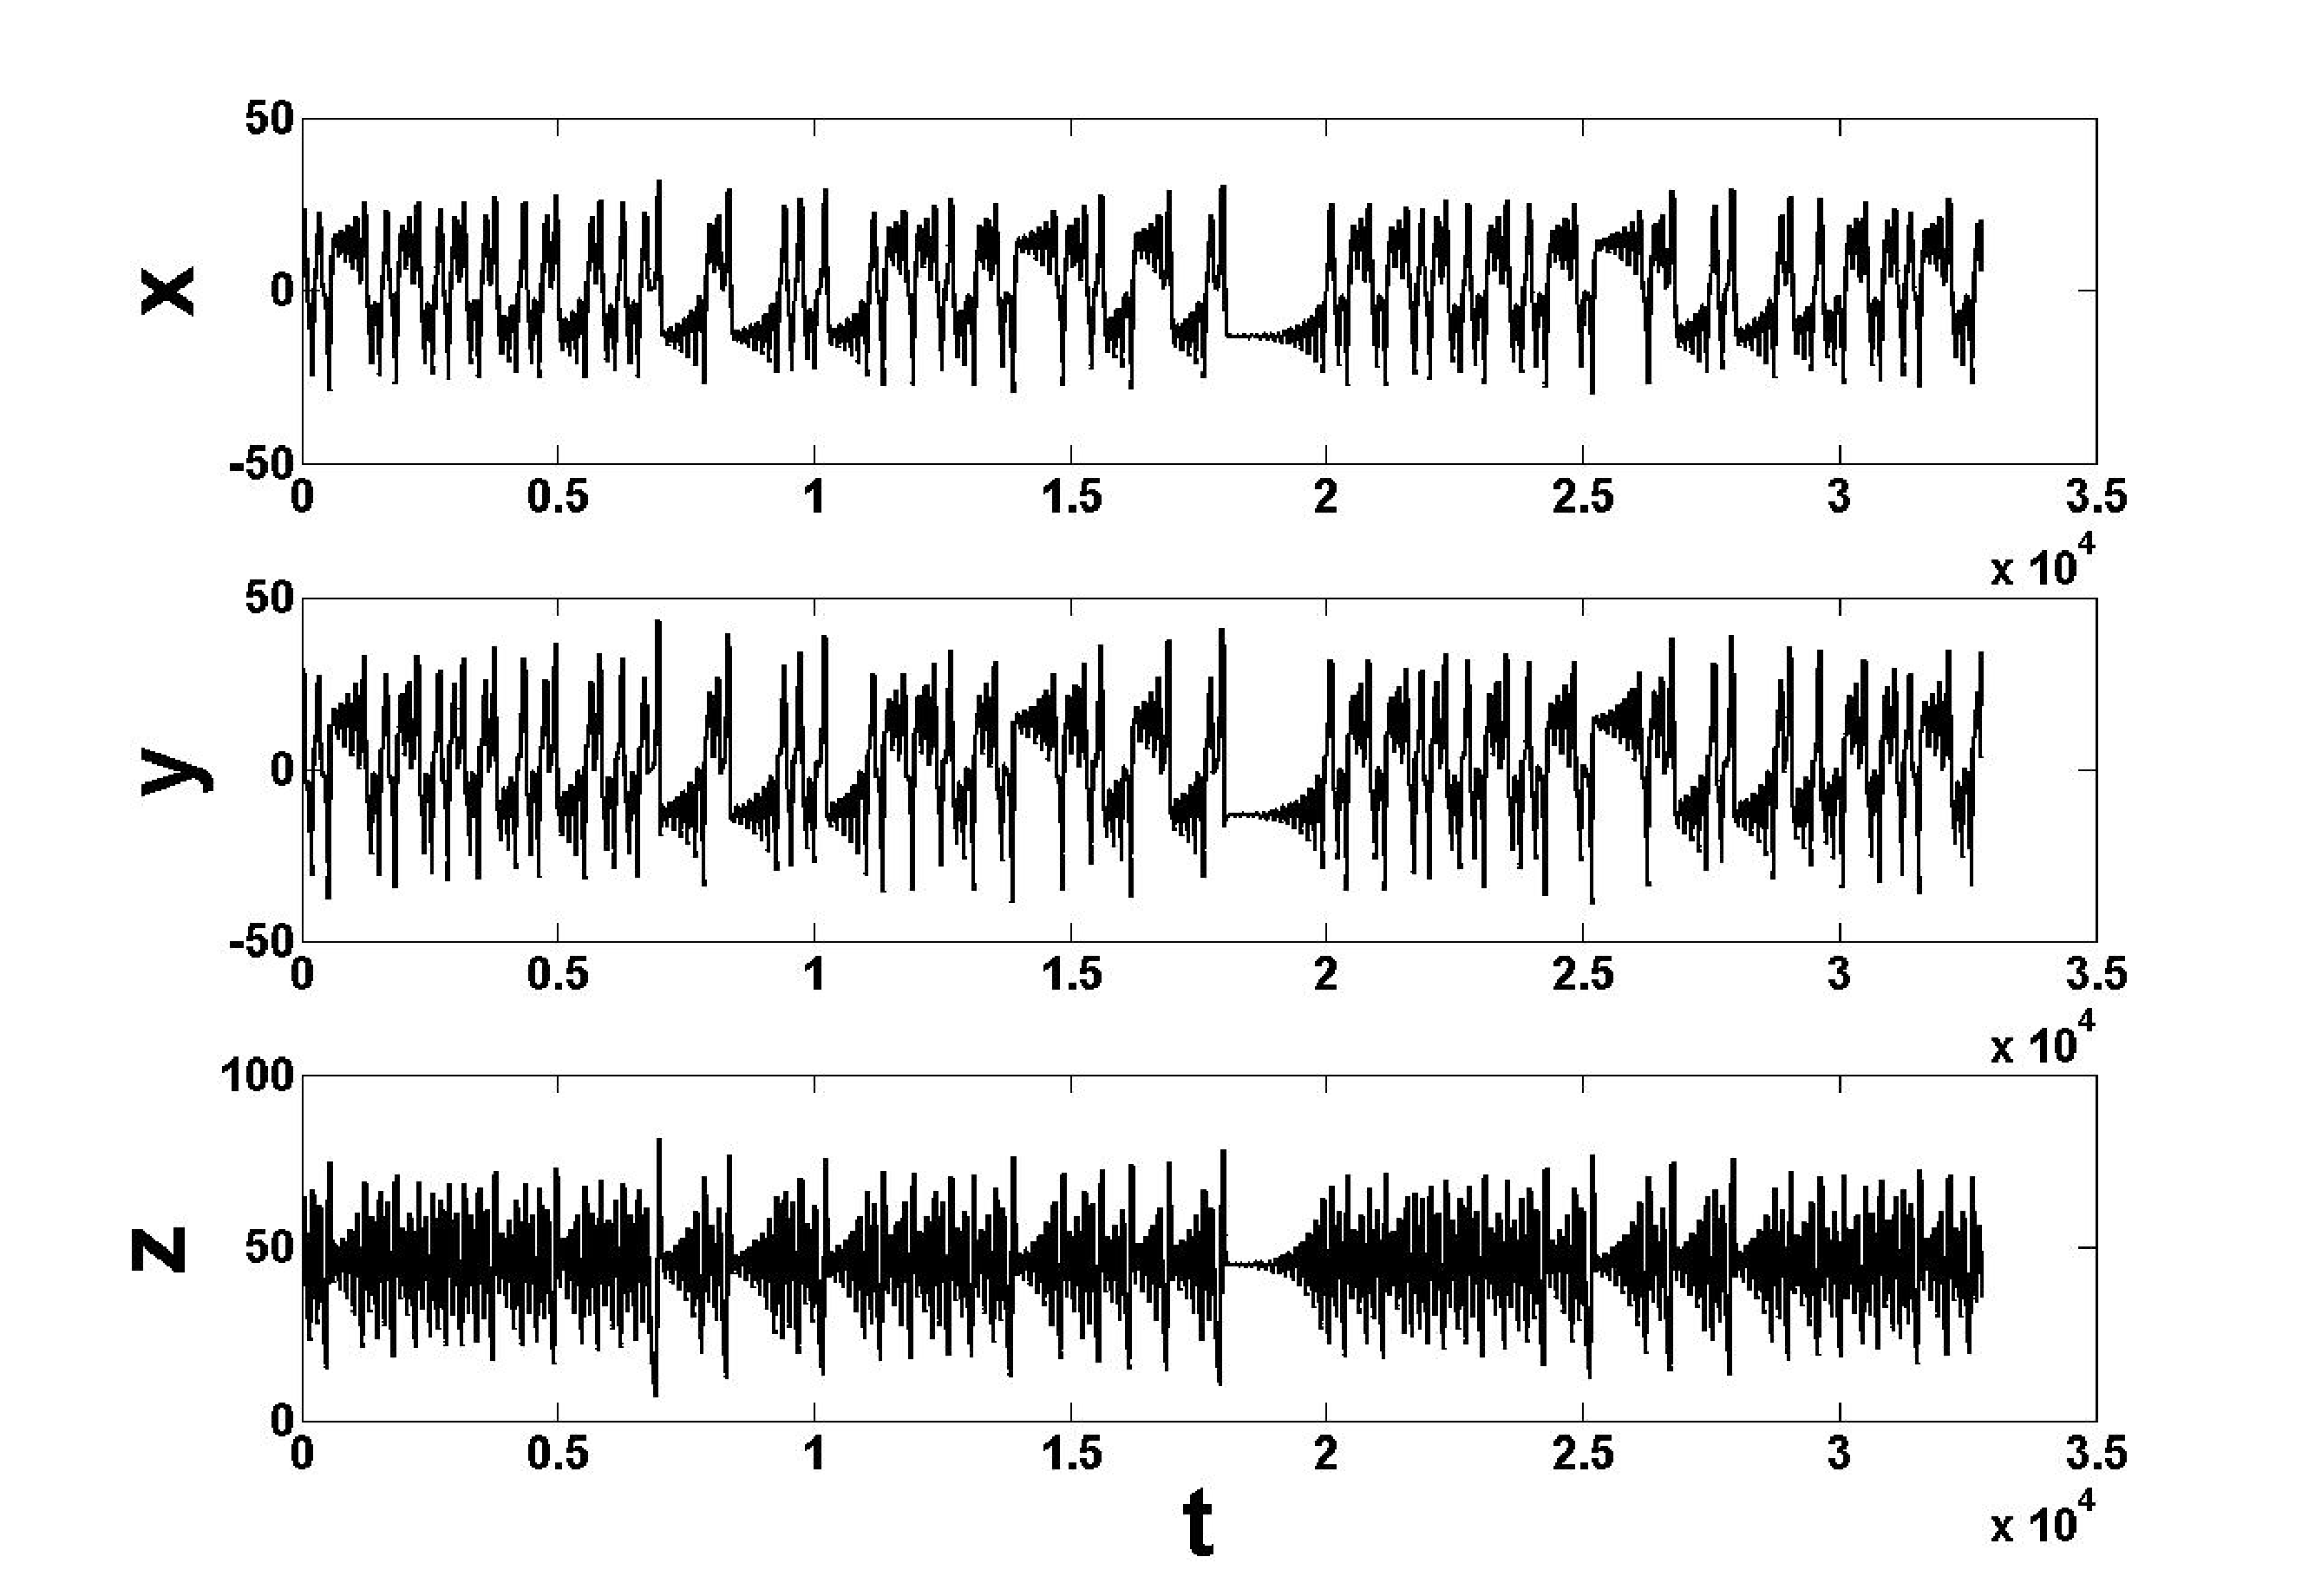
\includegraphics[width=1\columnwidth]{LorenzTiempo.pdf}\\
	\caption{Lorenz time series.}\label{fig:tiempo}
\end{figure}
%
\begin{figure}
	\centering
	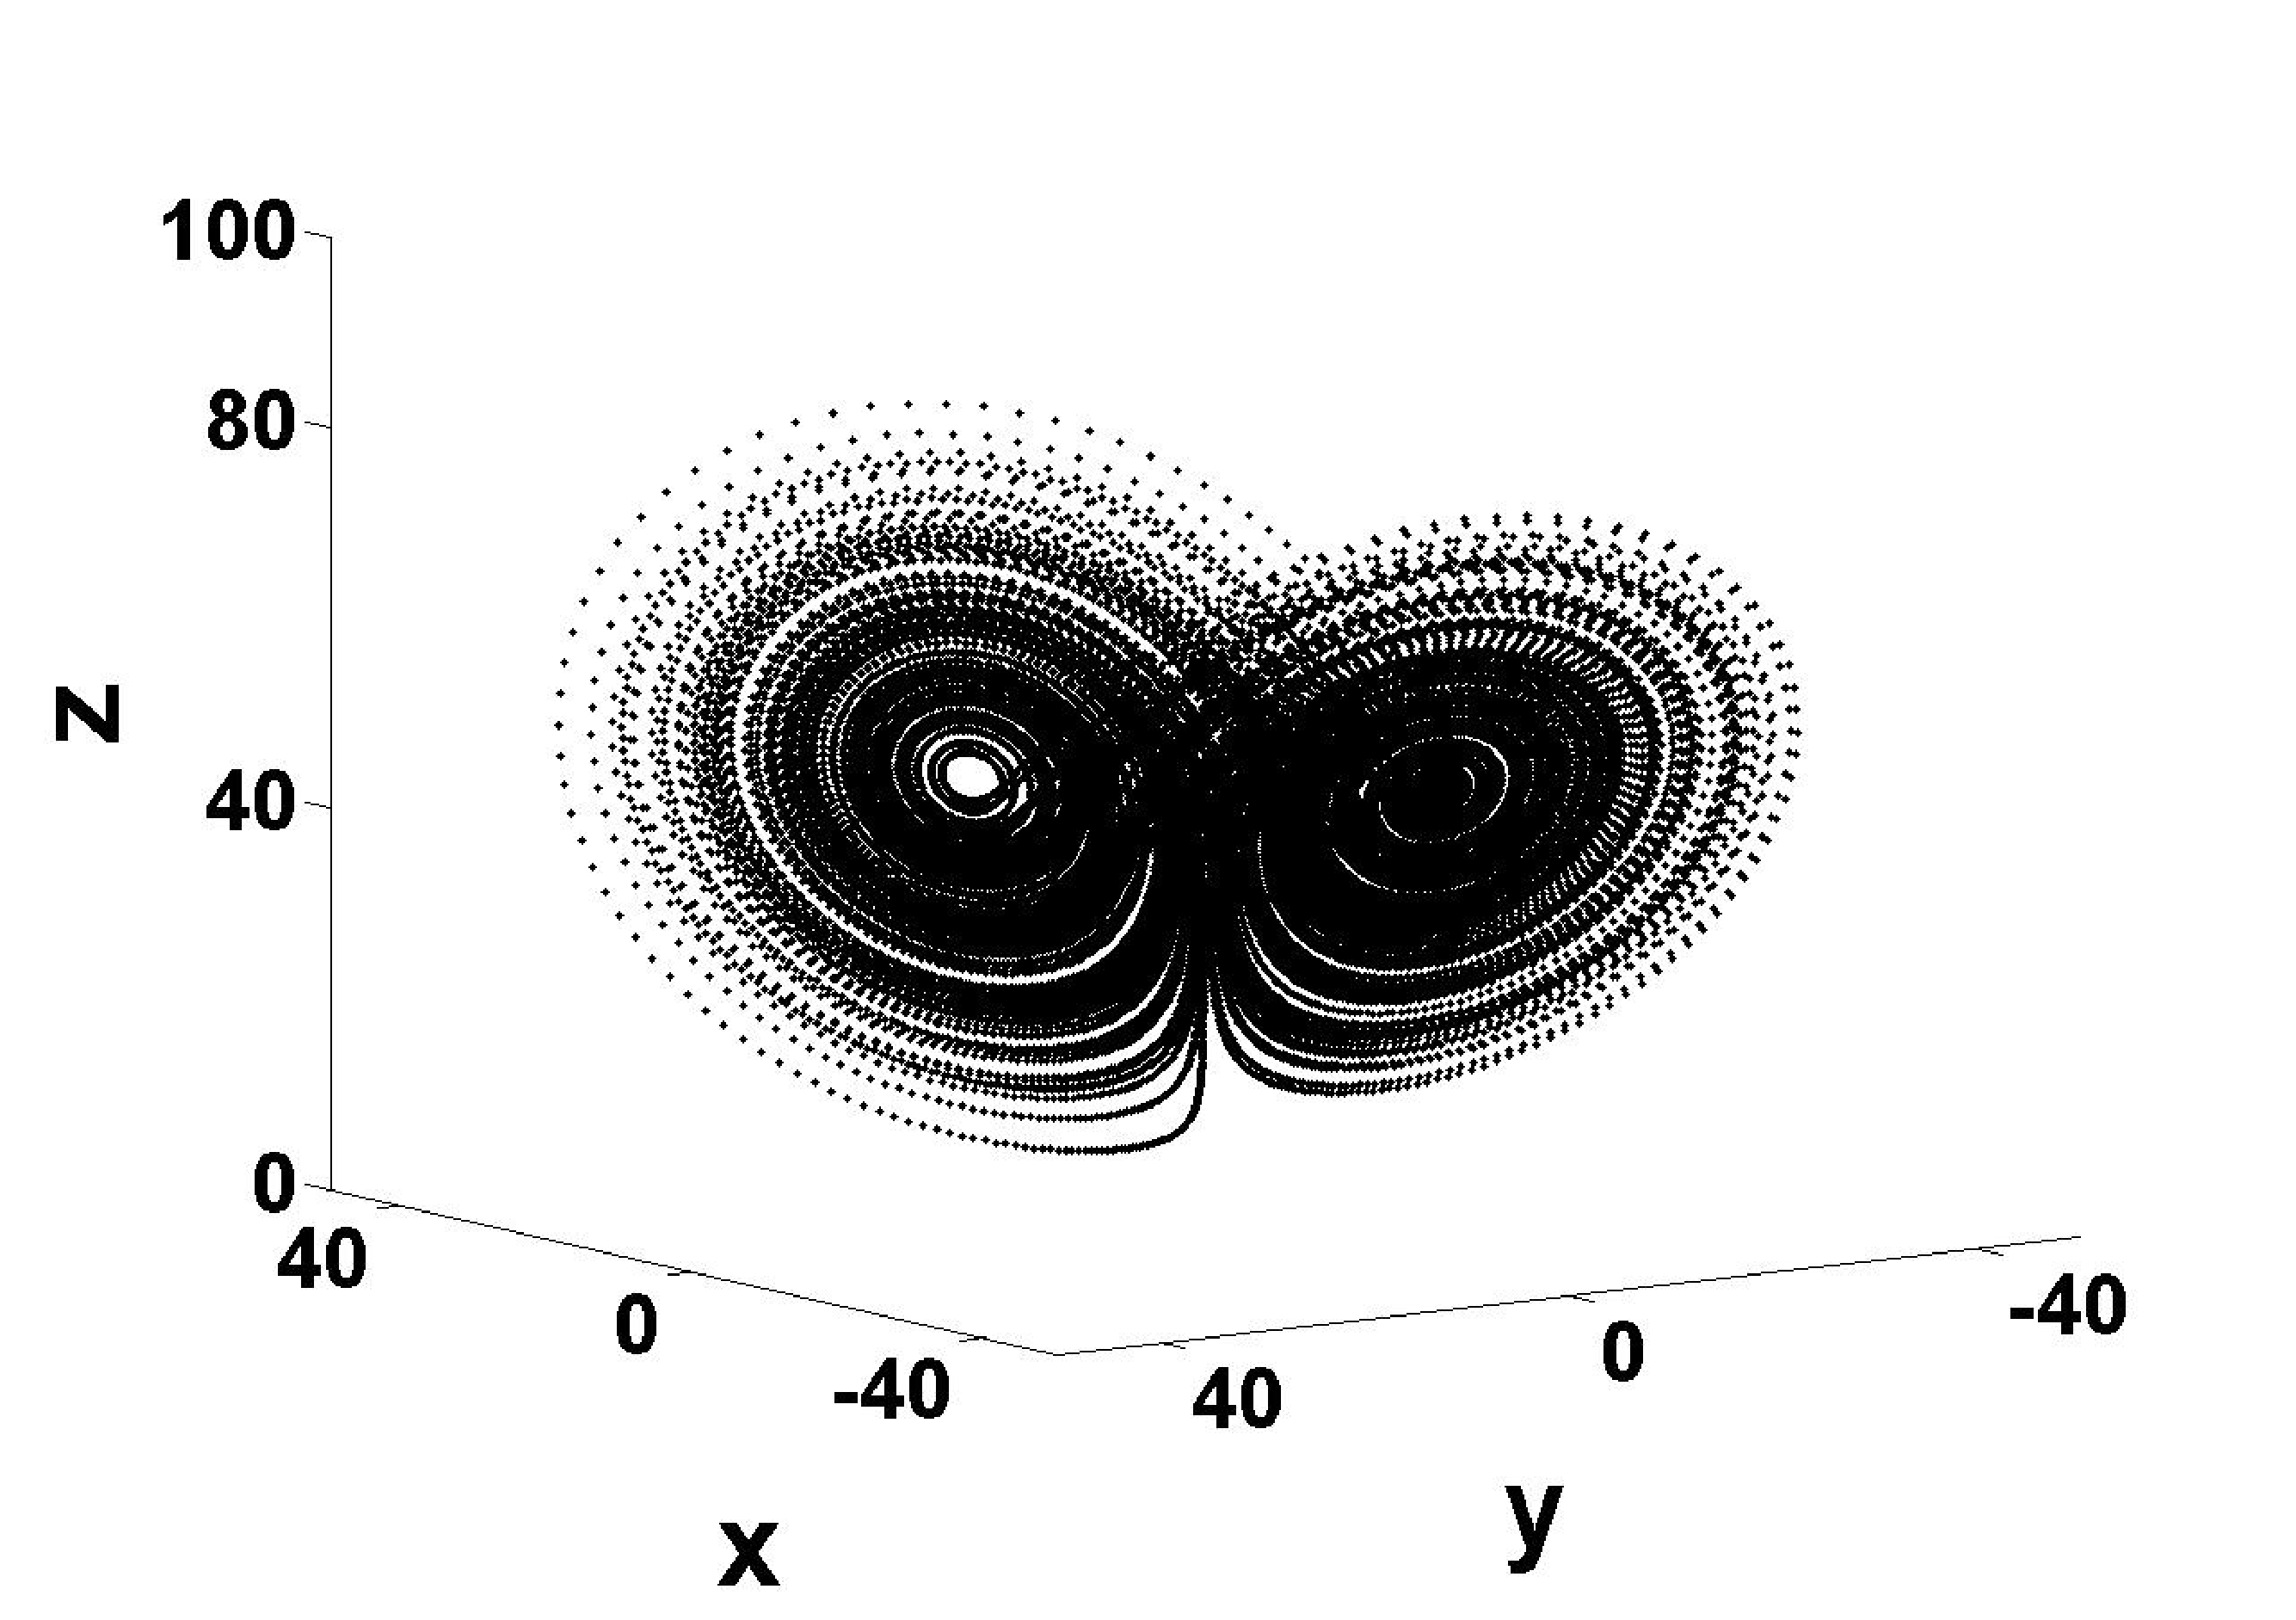
\includegraphics[width=1\columnwidth]{LorenzAtractor}\\
	\caption{Lorenz attractor.}\label{fig:atractor}
\end{figure}

In Table \ref{tabla:Tabla1} a comparison between the compilation results in the three numeric representations studied here:
\begin{itemize}
\item \textit{floating point arithmetics}: two cases, single and double precision (Float($32$bits) and Float($64$bits) respectively),
\item \textit{integer arithmetics} (Integer($54$bits)) and
\item \textit{fixed point arithmetics}: two cases, both with   $9$ bits for the integer part plus $1$ bit for the sign plus $22$ bits  (Fixed point($32$bits) or $54$ bits (Fixed point($64$bits)) respectively, for the fractional part.
\end{itemize}

The hardware required is shown in Table \ref{tabla:Tabla1}.
The integer arithmetic implementation is the one that employs minimum resources and supports a higher $f_{max}$, the reason for this is that the equations implemented were previously optimized for this particular application.
In the case of floating point representation optimization was made to diminish the area but other optimization techniques may be applied to improve frequency, or power consumption \cite{Giri2012,Gokul2004}.

\begin{table*} [tb]
\begin{center}
\caption{Compilation results CYCLONE III  EP3C120F780C7.}
\begin{tabular}{|c|c|c|c|c|c|c|c|}
\hline\hline
									&Fixed point($32$bits)	&Fixed point($64$bits)	&Float($32$bits)	&Float($64$bits)	&Integer($54$bits)  \\
\hline\hline
Total logic elements				&$2,392$    			&$6,104$     			&$8,176$   			&$17,532$  			&$1,297$			\\
\hline
Percentage of logic elements [\%] 	&$2.00$					&$5.12$     			&$6.86$            	&$14.72$          	&$1.08$   			\\
\hline
Total registers                  	&$1,658$            	&$1,754$       			&$4,753$     		&$8,532 $        	&$159$ 				\\
\hline \hline
clk $f_{max}$ [MHz]         		&$37.82$         		&$20.51$      			&$7.48$          	&$5.42$     		&$55.38$ 			\\
\hline
Throughput [Mbs]       				&$1,210.24$ 			&$656.32$         		&$14.96$          	&$173.44$          	&$1,772.16$   		\\
\hline\hline
\end{tabular}\end{center}
\label{tabla:Tabla1}
\end{table*}

In order to employ this system as a hardware PRNG output data are processed with \textit{discarding} and \textit{concatenating} techniques. 
Both techniques keep the least significant bits because they present the more variable behavior.
In the case of \textit{concatenating} technique, the noisiest part of each state variable is kept and recombined, and a $32$-bits sequence output is obtained in each iteration.

For the stochasticity analysis data files with $3,000,000$ $32$-bits words each were generated for $\Delta t=2^{-n}$, with $n=6$,$7$,$8$,$9$ and $10$.
DIEHARD tests were calculated for all the files generated.
In Table \ref{tabla:Tabla2} some of the most relevant results are reported.
$x_{disc}$, ( $y_{disc}$, $z_{disc}$) means $x$-time series ($y$, $z$) after the discarding randomization technique is applied.
$xyz$ means the time series obtained by means of the \textit{concatenating} randomization technique.
This Table \ref{tabla:Tabla2} shows that in the cases of integer and fixed point implementations the discarding randomization technique works better as $\Delta t$ increases because, for lower $\Delta t$ consecutive elements in the time series are more correlated and this randomization technique does not mix them enough.
In order to use lower values of  $\Delta t$ more bits should be discarded to obtain good PRNGs.
On the other hand the concatenating randomization technique performs well regardless of the value of $\Delta t$ (within the analyzed range).

\begin{table*} [tb]
\begin{center}
\caption{DIEHARD tests results.}
\begin{tabular}{|c|c|c|c|c|c|c|}
\hline\hline
						& $\Delta t=1/2^n$	&0,015625	&0,0078125	&0,00390625	&0,001953125	&0,0009765625	\\
\hline\hline
Float ($64$ bits)		&$x_{disc}$			&no    		&no    		&yes  		&yes 			&no  			\\
\hline
						&$y_{disc}$    	 	&no      	&no       	&yes    	&yes  			&no 			\\
\hline
						&$z_{disc}$   		&yes     	&yes       	&yes    	&no 			&no				\\
\hline
						&$zyx$             	&no   		&no      	&no        	&no 			&yes 			\\
\hline\hline
Fixed Point ($64$ bits)	&$x_{disc}$       	&yes    	&yes      	&no    		&no  			&no    			\\
\hline
						&$y_{disc}$        	&yes       	&yes    	&no     	&no  			&no    			\\
\hline
						&$z_{disc}$      	&yes     	&yes    	&no    		&no  			&no    			\\
\hline
						&$zyx$            	&yes    	&yes    	&yes   		&no  			&no    			\\
\hline\hline
Integer ($54$ bits)		&$x_{disc}$     	&yes   		&yes  		&no  		&no  			&no    			\\
\hline
						&$y_{disc}$       	&yes   		&yes     	&no  		&no  			&no    			\\
\hline
						&$z_{disc}$  		&yes 		&yes    	&no			&no  			&no    			\\
\hline
						&$zyx$       		&yes  		&yes 		&yes  		&yes 			&yes  			\\
\hline
\end{tabular}\end{center}
\label{tabla:Tabla2}
\end{table*}

\subsection{Conclusions}
\label{sec:conclusions} From the results presented herein, it is possible to conclude that to obtain a PRNG optimum results correspond to the integer arithmetics representation in both hardware (resources and frequency) and statistical properties.
The \textit{concatenating} randomization technique makes the quality independent of $\Delta t$ for this numeric representation.
For \textit{discarding} randomization technique good results are obtained  only for big values of $\Delta t$.
The same happens for fixed point implementations with both randomization techniques.

In terms of usage resources and frequency limitations integer arithmetics performance is considerable better than floating point and fixed point.
Let us remark that to minimize resources preprocessing of the chaotic system is required (scaling and polarization) to get dividers that are a power of $2$, as explained in subsection \ref{sec:impleInt}.

On the other hand, for the floating point arithmetic's case the exponent is discarded in all the used randomization techniques and consequently the dynamics is highly perturbed by the randomization process.
Then, as shown in Table \ref{tabla:Tabla2} $\Delta t$ is not the relevant variable to predict a good or a bad PRNG.